\section{Introduction} \label{introduction}
%% General Introduction
Machine learning techniques are increasingly being used in industrial and scientific applications to gain insight from the data.
Typically, a machine learning pipeline is a series of complex data processing steps to process a labeled training dataset and produce a machine learning model.
The machine learning model is then used to make predictions on new unlabeled data.
To fully utilize the model, it has to be deployed into an environment where it can answer prediction queries in real-time.

%% Intro to the problem of continuous improvement
After the model is deployed, new training data may become available.
In order to adapt to the new training data, one has to retrain and redeploy the model.
In many real-world use cases, training datasets are very large which may require hours of data preprocessing and training to result in a new model.
Therefore, it is not feasible to train a new model frequently.
This means that the deployed model is not always up-to-date.
Online learning methods are utilized to provide fresh and up-to-date models.
However, unless the online learning method is highly tuned to the specific use case, it does not guarantee a high prediction accuracy \cite{ma2009identifying, macmahan2013}. 
This results in a trade-off between the model training cost and the model quality.
Moreover, any incoming prediction and training data has to be first preprocessed by the same pipeline that was used during the initial training. 
Therefore, deploying models alone are not adequate and the entire pipeline has to be deployed as well.

%% Current Deployment Systems
Several existing platforms such as Velox, Clipper, TensorFlow Extended provide support for deployment of models with TensorFlow Extended being the only one that supports deployment of the entire machine learning pipeline \cite{crankshaw2014missing, crankshaw2016clipper, agarwal2014laser, baylor2017tfx}.
However, the existing systems only support online learning, periodical retraining, or a combination of the two for maintaining the quality of models.
In many cases, the amount of training data is very large, thus training a new pipeline may take hours (or even days) \cite{baylor2017tfx}.
During the retraining, incoming prediction requests are answered by the old model and new real-time training data are accumulated.
By the time the retraining is finished, enough data is accumulated to prompt for a new round of training.
As a result, in the current deployment platforms, the deployed models and pipelines are constantly out of date which results in lower prediction accuracy.

%% Use case
\begin{figure}[h!]
\centering
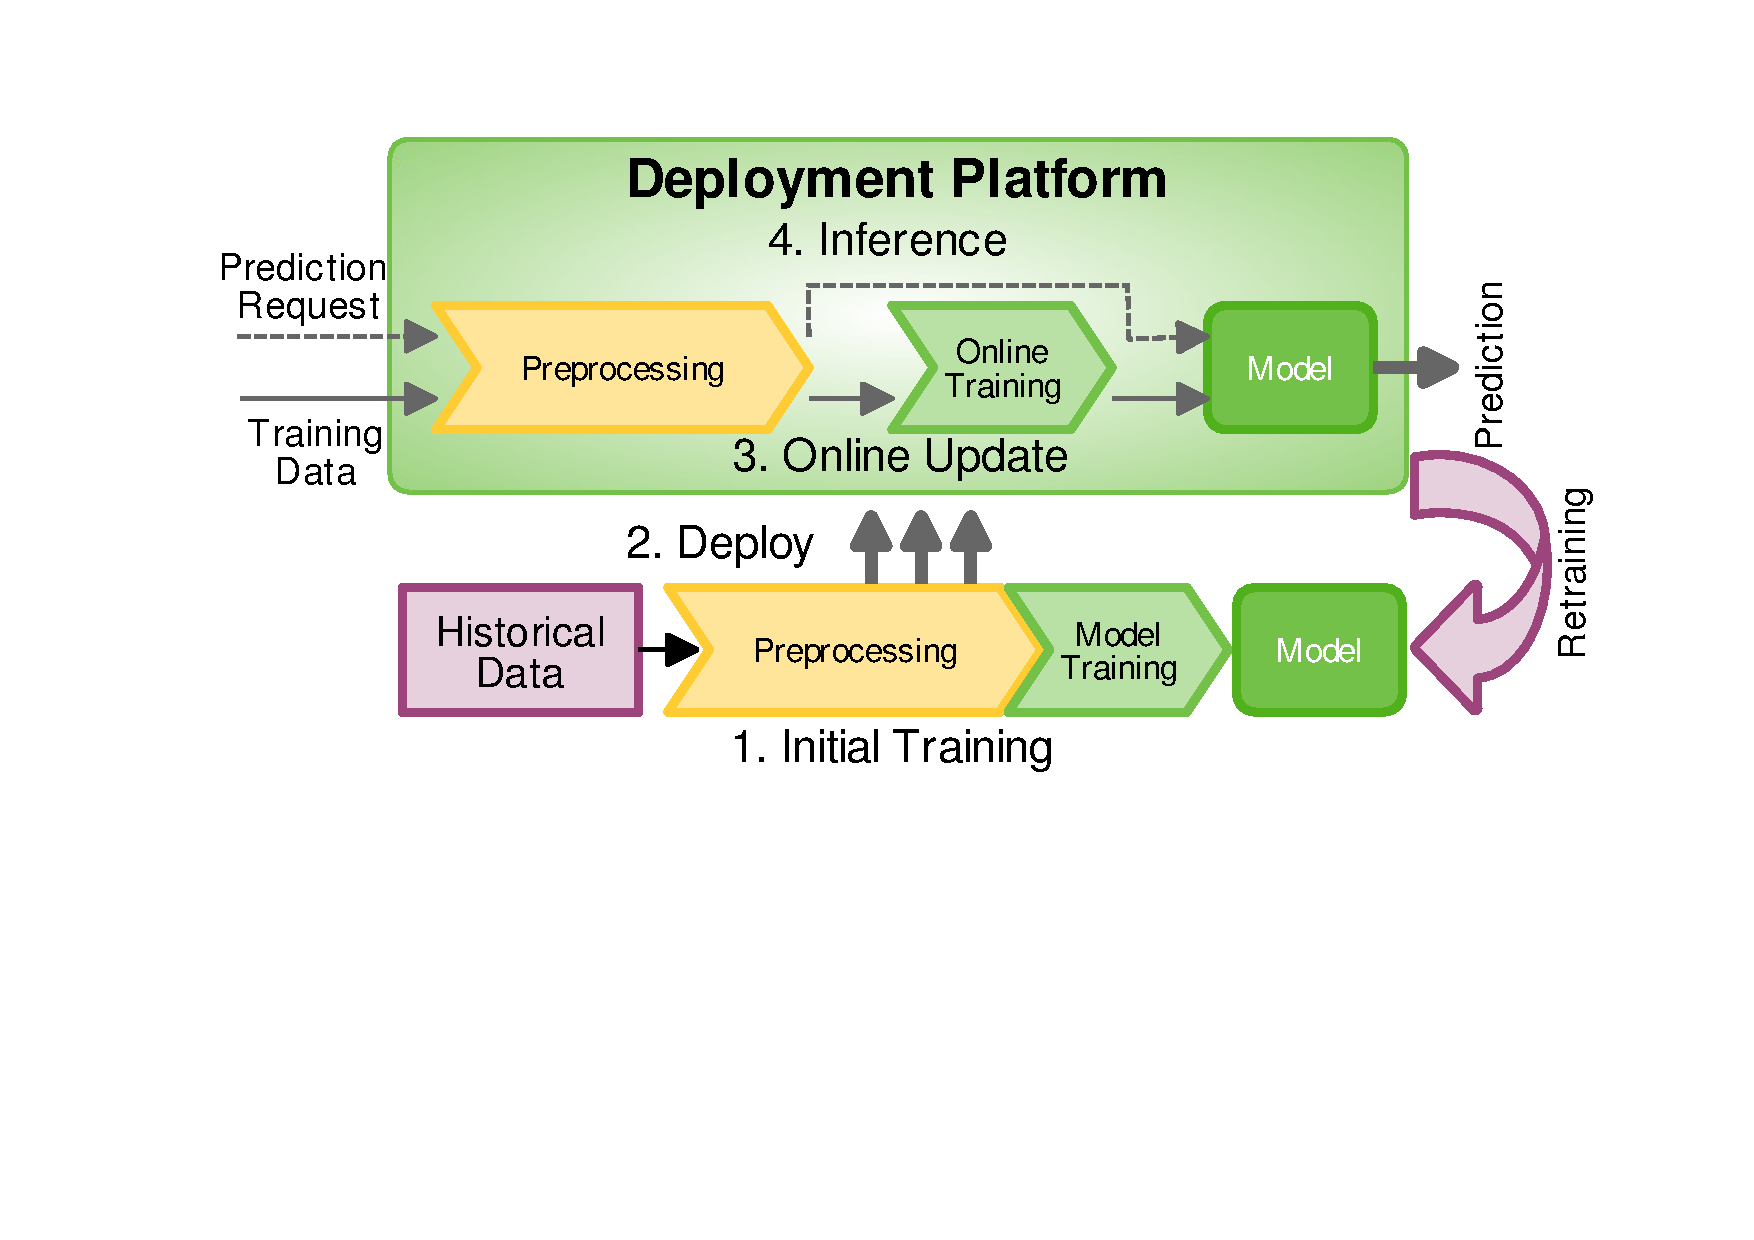
\includegraphics[width=\columnwidth]{../images/generic-motivational-example-v2.pdf}
\caption{Deployment process of machine learning pipelines}
\label{fig:motivational-example}
\end{figure}

Figure \ref{fig:motivational-example} shows the typical deployment process of existing systems.
From an existing dataset, a pipeline consists of several data and feature processing steps, and a training algorithm is trained \textcircled{1}.
Then, the deployment platform deploys the model (with the pipeline) \textcircled{2}.
Prediction requests arrive at the deployment platform \textcircled{3} where first they are transformed into an unlabeled data point (by request processor) and then they are forwarded to the pipeline.
The pipeline first transforms the unlabeled data into a set of features and then the model makes a prediction based on the feature values  \textcircled{4}.
The resulting predictions are further processed and converted to meaningful actions before being presented back to the users or the entities issuing the prediction queries \textcircled{5}.
Based on the result of the prediction query, feedback, containing the original prediction query and the correct label, may be generated that is appended to the existing training data \textcircled{6}.
The deployment platform also uses the feedback data to further update the model using online learning methods \textcircled{7}.
The deployment platform also provides statistics such as the prediction accuracy over time and rate of the incoming predictions and training data.
Throughout the deployment process, it is possible that the accuracy of the predictions being made drop below an acceptable threshold due to the changes in the distribution of the incoming prediction requests.
As a result, the model and the pipeline are regularly retrained and redeployed back into the deployment platform(\textcircled{1} to \textcircled{7} is repeated).

Several real-world use cases follow the workflow described in Figure \ref{fig:motivational-example}.
One example is the problem of Ad click prediction \cite{macmahan2013}.
In Ad click prediction, the machine learning pipeline typically consists of extracting features from the users and ads. 
Logistic regression models have shown to perform well in this setting \cite{macmahan2013}.
Prediction queries consist of the user's information and a pool of available ads for displaying to the user.
Once a prediction score for each of these ads are made, an Ads selector unit (similar to the Prediction Processor in Figure \ref{fig:motivational-example}) picks a set of ads with the highest score to display to the user.
Based on the action of the user (click or no click), new training data, containing the original prediction request and the label (+1 for a clicked ad and -1 for a non-clicked ads) will be generated which is stored with the existing training data (similar to the Feedback Generator in the Figure).
\hl{maybe another use case (IoT or Steel coil flatness prediction)}

The above example demonstrates the complexity of deployment and maintenance of machine learning pipelines through offline retraining.
A flexible deployment platform should, therefore, be able to meet the model quality requirement without requiring the periodical offline retraining of the models and pipelines.

%% Our solution
We propose a deployment platform that continuously updates the model (and the pipeline) using a combination of the historical and incoming data.
Our deployment platform updates the model using the incoming feedback data (we call this the real-time training data) similar to how online machine learning algorithms work while simultaneously performs small batch updates using the historical data.
Our deployment platform offers two key optimizations.

\textit{Proactive training.}
Instead of periodically training a new model using the historical training data, we continuously update the existing model using random batches sampled from the historical data.
In proactive training, the deployment platform processes the batch using the pipeline first, and then it updates the model.
The updated model is immediately ready for answering prediction queries.
Our experiments show that proactive training of the model achieves more accurate predictions over time and requires fewer resources when compared to the periodical retraining.

\textit{Online Statistics Computation and Feature Materialization.}
Our deployment platform employs advanced online learning methods (such as Adagrad \cite{duchi2011adaptive}) to update the model in real-time, before storing data.
Before the model is updated, the pipeline has to process the real-time data.
First, the pipeline computes the necessary statistics required by each component (such as feature mean and feature standard deviation for scaling the data).
Then, the pipeline transforms the data into a set of features for updating the model. 
The deployment platform stores the updated statistics for every pipeline component and materializes the transformed features by storing them in memory or disk.
By reusing the computed statistics and the materialized features during the proactive training, we are able to decrease the proactive training time by 50\%.

% Our contributions
In summary, our contributions are:
\begin{itemize}
\item A platform for continuously training deployed machine learning models and pipelines that adapts to the changes in the incoming data.
\item Proactive training of the deployed models and pipelines that frequently updates the model in-place using a combination of the historical and the real-time data and increases the prediction accuracy when compared with state of the art.
\item Efficient pipeline processing and model training by online statistics computation and feature materialization, thus guaranteeing the availability of up-to-date models for answering prediction queries.
\end{itemize}

The rest of this paper is organized as follows:
Section \ref{continuous-training-serving} describes the details of our continuous training approach.
In Section \ref{sec:system-architecture}, we introduce the architecture of our deployment system.
In Section \ref{evaluation}, we evaluate the performance of our continuous deployment approach.
Section \ref {related-work} discusses the related work.
Finally, Section \ref{conclusion} presents our conclusion and the future work.
